\documentclass[usenames,dvipsnames]{beamer}
    \mode<presentation> {
    \usetheme{Montpellier}
    \useoutertheme{tree}
    \usecolortheme{beaver}
    %\setbeamertemplate{footline} % To remove the footer line in all slides uncomment this line
    \setbeamertemplate{footline}[page number] % To replace the footer line in all slides with a simple slide count uncomment this line
    \setbeamertemplate{navigation symbols}{} % To remove the navigation symbols from the bottom of all slides uncomment this line
    \setbeamersize{text margin left=8mm,text margin right=5mm}
    }

    \usepackage{graphicx} % Allows including images
    \usepackage{booktabs} % Allows the use of \toprule, \midrule and \bottomrule in tables
    %\usepackage[outputdir=target]{minted}
    \usepackage{minted}
    \usepackage{xcolor}
    \usepackage[utf8]{inputenc}
    \usepackage{pifont}
    \usepackage{xspace}
    \usepackage{newunicodechar}
    \newunicodechar{✪}{\ding{74}}

    \definecolor{mintedbackground}{rgb}{0.95,0.95,0.95}
    \newcommand{\code}[1]{\colorbox{lightgray}{\texttt{#1}}}
    \newcommand{\distage}{\texttt{distage}\xspace}

\newminted{scala}{
    bgcolor=mintedbackground,
    fontfamily=tt,
    linenos=true,
    numberblanklines=true,
    numbersep=5pt,
    gobble=0,
    frame=leftline,
    framerule=0.4pt,
    framesep=2mm,
    funcnamehighlighting=true,
    tabsize=4,
    obeytabs=false,
    mathescape=false
    samepage=false, %with this setting you can force the list to appear on the same page
    showspaces=false,
    showtabs =false,
    texcl=false,
}

\newminted{text}{
    bgcolor=mintedbackground,
    fontfamily=tt,
    linenos=true,
    numberblanklines=true,
    numbersep=5pt,
    gobble=0,
    frame=leftline,
    framerule=0.4pt,
    framesep=2mm,
    funcnamehighlighting=true,
    tabsize=4,
    obeytabs=false,
    mathescape=false
    samepage=false, %with this setting you can force the list to appear on the same page
    showspaces=false,
    showtabs =false,
    texcl=false,
}

\newminted{json}{
    bgcolor=mintedbackground,
    fontfamily=tt,
    linenos=true,
    numberblanklines=true,
    numbersep=5pt,
    gobble=0,
    frame=leftline,
    framerule=0.4pt,
    framesep=2mm,
    funcnamehighlighting=true,
    tabsize=4,
    obeytabs=false,
    mathescape=false
    samepage=false, %with this setting you can force the list to appear on the same page
    showspaces=false,
    showtabs =false,
    texcl=false,
}

    \setminted{fontsize=\footnotesize,baselinestretch=1}

    \usepackage{tikz}
    \usetikzlibrary{positioning}
    %\graphicspath{{target/media/}}

    \title[\distage]{\distage: Modern Staged Dependency Injection for Scala}

    \institute[Septimal Mind Ltd]
    {
    Septimal Mind Ltd\\
    \medskip
    \textit{team@7mind.io}
    }
    \date{\today}

\makeatletter
\setbeamertemplate{headline}
{%
    \begin{beamercolorbox}[wd=\paperwidth,colsep=1.5pt]{upper separation line head}
    \end{beamercolorbox}
    \begin{beamercolorbox}[wd=\paperwidth,ht=2.5ex,dp=1.125ex,%
      leftskip=.3cm,rightskip=.3cm plus1fil]{title in head/foot}
      \usebeamerfont{title in head/foot}\insertshorttitle
    \end{beamercolorbox}
    \begin{beamercolorbox}[wd=\paperwidth,ht=2.5ex,dp=1.125ex,%
      leftskip=.3cm,rightskip=.3cm plus1fil]{section in head/foot}
      \usebeamerfont{section in head/foot}%
      \ifbeamer@tree@showhooks
        \setbox\beamer@tempbox=\hbox{\insertsectionhead}%
        \ifdim\wd\beamer@tempbox>1pt%
          \hskip2pt\raise1.9pt\hbox{\vrule width0.4pt height1.875ex\vrule width 5pt height0.4pt}%
          \hskip1pt%
        \fi%
      \else%
        \hskip6pt%
      \fi%
      \insertsectionhead
      \usebeamerfont{subsection in head/foot}%
      \ifbeamer@tree@showhooks
        \setbox\beamer@tempbox=\hbox{\insertsubsectionhead}%
        \ifdim\wd\beamer@tempbox>1pt%
          \ \raise1.9pt\hbox{\vrule width 5pt height0.4pt}%
          \hskip1pt%
        \fi%
      \else%
        \hskip12pt%
      \fi%
      \insertsubsectionhead\hfill\insertframenumber/\inserttotalframenumber\hspace{0.5em}
    \end{beamercolorbox}
    \begin{beamercolorbox}[wd=\paperwidth,colsep=1.5pt]{lower separation line head}
    \end{beamercolorbox}
}
\makeatother

\begin{document}

% \begin{VerbatimOut}{ex-scala-roles.tmp}
% @RoleId("testservice")
% class TestService[F[_] : Monad](http: HttpSrv[F])
%   extends IzService {
%     override def start(): Unit = http.start()
%     override def stop(): Unit = http.stop()
% }
% class TestPlugin extends PluginDef {
%   many[IzService].add[TestService[IO]]
% }
% object TestLauncher {
%   // run with
%   // java test.jar test-service other-service
%   def main(args: Array[String]): Unit = IzRoleApp(args).main()
% }
% \end{VerbatimOut}

\begin{frame}
%\titlepage
\begin{figure}
\Huge
\color{RubineRed} dist✪ge
\noindent
\rule{\linewidth}{1mm}
\Large Modern Staged Dependency Injection for Scala
\rule{\linewidth}{1mm}
\end{figure}

\begin{figure}
\color{RubineRed}
\normalsize Modular Functional Programming \\
with \\
Context Minimization \\
through \\
Garbage Collection
\end{figure}



\begin{figure}
  Septimal Mind Ltd \\
  \textit{team@7mind.io} \\
  
\includegraphics[width=0.2\textwidth]{media/logo_7mind.png}
\end{figure}

\end{frame}

%%%%%%%%%%%%%%%%%%%%%%%%%%%%%%%%%%%%%%%%%%%%%%%%%%%%%%%%%%%%%%%%%%%%%%%%%%%%%%%%%%%%%%%%%%%%%%%%%%%
\section{The argument: Dependency Injection vs. Functional Programming}

\begin{frame}
\frametitle{DI is outdated and doesn't compose with FP?}
  Many Scala folks think that:
  \begin{enumerate}
  \item DI is heavy and slow
  \begin{itemize}
    \item \textit{``tests start longer than they run''}
  \end{itemize}
  \item DI is unsafe
  \begin{itemize}
    \item \textit{``my program compiles but crashes at runtime after a huge delay''}
  \end{itemize}
  \item DI doesn't work for modern FP code
  \begin{itemize}
    \item \textit{``we cannot inject \code{IO\lbrack\_, \_\rbrack} into \code{Repository\lbrack\_\lbrack\_, \_\rbrack\rbrack}''}
  \end{itemize}
  \item DI is full of magic and error-prone
  \begin{itemize}
    \item \textit{``I've read 80\% of the 5000-page Spring manual but still don't understand why I need to put these 12 annotations here.
    I've tried Guice but it failed with 10-megabyte stacktrace after five minutes and 300 retries of database connection initialization''}
  \end{itemize}
  \end{enumerate}
\end{frame}

%\begin{frame}
%\frametitle{DI is outdated and doesn't compose with FP?}
%  \center{
%  \textit{``Given its native support for type classes and higher-kinded types -- both features indispensable to functional programming -- DI Stage is one of the leading dependency injection libraries out there. Bonus points for being built by a wicked-smart team that contributes to ZIO!''}
%  }
%  \newline
%  \leftline{\textit{ --– John A. De Goes}}
%\end{frame}

\begin{frame}[fragile]
\frametitle{TLDR}
  \begin{scalacode}
import distage._, scalaz.zio.IO

trait Repository[F[_, _]]
class ProductionRepository[F[_, _]] extends Repository[F]
class DummyRepository[F[_, _]] extends Repository[F]
class App[F[_, _]](repository: Repository[F]) { def run = ??? }

class MyAppProd[F[_, _]: TagKK] extends ModuleDef {
  make[Repository[F]].from[ProductionRepository[F]]
  make[App[F]]
}
class Main[F[_, _]: TagKK: BIO] extends App {
  Injector()
    .produceF[F[Throwable, ?]](
      new MyAppProd[F], roots=Set(DIKey.get[App[F]])
    ).use(_.get[App[F]].run)
}
object Main extends Main[IO]
  \end{scalacode}
\end{frame}

%%%%%%%%%%%%%%%%%%%%%%%%%%%%%%%%%%%%%%%%%%%%%%%%%%%%%%%%%%%%%%%%%%%%%%%%%%%%%%%%%%%%%%%%%%%%%%%%%%%
\section{\distage{} features}
\begin{frame}
  \frametitle{\distage: overview}
  \begin{enumerate}
    \item Staging: \textit{plan all the work before you do anything},
    \item Garbage Collection: \textit{instantiate reachable instances only},
    \item Higher-Kinded Types: \textit{inject typeclass instances, use parametricity},
    \item Path-Dependent Types support,
    \item Lifecycle and Resources: \textit{inject any cats.effect.Resource[F, A]},
    \item Plan introspection: \textit{graphviz, text dump, dependency trees},
    \item Plan rewriting,
    \item Roles: \textit{multiple services in one process},
    % \item Sets: \textit{collect listeners, hooks, routes...}
    \item Dynamic Plugins\footnotemark[1] and Testkit,
    \item Circular Dependencies support,
    \item Assisted Injection and Trait Augmentation\footnotemark[2],
    \item Automatic Sets: \textit{prepopulate sets with all instances of a class}
  \end{enumerate}
  \footnotetext[1]{Runtime with compile-time verification}
  \footnotetext[2]{Runtime or compile-time generation}
\end{frame}

\begin{frame}
\frametitle{Garbage Collection for better and faster tests}
  \begin{enumerate}
    \item Define all your test and production dependencies as a flat list,
    \item Put discrimination tags on test-specific definitions,
    \item Only the instances required for your tests will be instantiated,
    \item Creation takes milliseconds, not like in Spring,
    \item $\Rightarrow$ Significant savings on test startup time.
    \item You don't need to setup your context, it's done automatically by Plugin Loader and Garbage Collector,
    \item $\Rightarrow$ Substantial savings on test setup boilerplate.
  \end{enumerate}
\end{frame}

\begin{frame}[fragile]
\frametitle{Example: Garbage Collection and tests}\begin{scalacode}
class ProductionRepository[F[_, _]] extends Repository[F]
class DummyRepository[F[_, _]] extends Repository[F]

class MyAppPlugin extends PluginDef {
  make[Repository[IO]].from[ProductionRepository[IO]]
  make[Repository[IO]].tagged("test").from[DummyRepository[IO]]
}
class RepoTest extends DistagePluginSpec {
  "repository" must {
    "work correctly" in diIO {
      (repository: Repository[IO]) => // repository is GC root
      // Repository is DummyRepository - "test" tag prioritized
      // ProductionRepository will not be instantiated!
      for { kv  <- randomIO[KeyValue]
            _   <- repository.put(kv)
            kv2 <- repository.get(kv.key)
      } yield assert(kv == kv2)
}}}
  \end{scalacode}
\end{frame}

\begin{frame}[fragile]
\frametitle{Garbage Collection for deployment: flexible monoliths}
  We may fuse Microservices with Monoliths keeping \textit{all} their benefits:
  \begin{enumerate}
  \item Develop services (\textit{Roles}\footnotemark[1]) separately, even in multirepo,
  \item Each Role is a Garbage Collection Root,
  \item Build a single Docker image with multiple Roles in it,
  \item Pass Roles you want to start as commandline parameters,
  \item $\Rightarrow$ higher computation density, savings on infrastructure,
  \item $\Rightarrow$ \textit{substantial} development simplification: full environment can be started on a low-end machine with one command.
  \end{enumerate}

  \begin{textcode}
server1# docker run company/product +analytics
server2# docker run company/product +accounting +users
developer1# docker run company/product +*
developer2# docker run company/product --dummy-repositories +*
  \end{textcode}

  \footnotetext[1]{Previous slides on the subject: https://goo.gl/iaMt43}
\end{frame}

\begin{frame}
\frametitle{Lifecycle}
  \begin{itemize}
    \item Applications manage a lot of global resources:
      \begin{enumerate}
      \item Connection pools, thread pools
      \item Servers, external endpoints, databases
      \item Configurations, metrics, heartbeats
      \item External log sinks
      \end{enumerate}
    \item They have to be started and closed in integration tests,
    \item We shouldn't set them up manually for every test,
    \item We want to create reusable components that correctly share a single resource.
  \end{itemize}
\end{frame}

\begin{frame}[fragile]
\frametitle{Lifecycle: \code{.fromResource}}
  \begin{enumerate}
    \item Inject any cats-effect Resource
    \item Global resources deallocate when the app or test ends
  \end{enumerate}

  \begin{scalacode}
object App extends IOApp {
  val blazeClientModule = new ModuleDef {
    make[ExecutionContext].from(ExecutionContext.global)
    addImplicit[Bracket[IO, Throwable]]

    make[Client[IO]].fromResource { ec: ExecutionContext =>
      BlazeClientBuilder[IO](ec).resource
  }}

  def run(args: List[String]): IO[ExitCode] =
    Injector().produceF[IO](blazeClientModule)
    .use { // Client allocated
      _.get[Client[IO]].expect[String]("https://google.com")
    }.as(ExitCode.Success) // Client closed
}
  \end{scalacode}
\end{frame}

\begin{frame}[fragile]
\frametitle{Effectful creation: \code{.fromEffect}}
  Global mutable state must be created effectfully, but doesn't have to be deallocated. e.g. a global parallelism limiter:

  \begin{scalacode}
    import distage._, import scalaz.zio._

    case class UploadConfig(maxParallelUploads: Long)

    class UploaderModule extends ModuleDef {
      make[Semaphore].named("upload-limit").fromEffect {
        conf: UploadConfig @ConfPath("myapp.uploads") =>
          Semaphore.make(conf.maxParallelUploads) }
      make[Uploader]
    }
    class Uploader(limit: Semaphore @Id("upload-limit")) {
      def upload(content: Content): IO[Throwable, Unit] =
        limit.withPermit(...)
    }
  \end{scalacode}
\end{frame}

\begin{frame}[fragile]
\frametitle{Config support}
  \distage has \texttt{HOCON} configuration extension.

  \begin{scalacode}
case class HostPort(host: String, port: Int)

class HttpServer(@ConfPath("http.listen") listenOn: HostPort) {
  // ...
}
  \end{scalacode}

  The extension:
  \begin{enumerate}
  \item Enumerates all the missing references in a Plan,
  \item Searches them for a specific \mintinline{scala}{@ConfPath} annotation,
  \item Tries to find corresponding sections in config source,
  \item Extends plan with config values,
  \item $\Rightarrow$ Config values are parsed before instantiation begins,
  \item $\Rightarrow$ Problems are shown quickly and all at once,
  \item $\Rightarrow$ Compile-time checker plugin validates config.
  \end{enumerate}
\end{frame}

\begin{frame}[fragile]
  \frametitle{Dynamic Plugins}
  Just drop your modules into your classpath:
  \begin{scalacode}
class AccountingModule extends PluginDef {
  make[AccountingService].from[AccountingServiceImpl]
  // ...
}
  \end{scalacode}
  Then you may pick up all the modules and build your context:
  \begin{scalacode}
val plugins = new PluginLoaderDefaultImpl(
  PluginConfig(Seq("com.company.plugins"))
).load()
// ... pass loaded modules to Injector
  \end{scalacode}
  \begin{enumerate}
  \item Useful while you are prototyping your app,
  \item In maintenance phase you may switch to static configuration.
  \end{enumerate}
\end{frame}

\begin{frame}
  \frametitle{Circular dependencies}
  \begin{enumerate}
    \item Supported via \texttt{Proxies},
    \item Cyclic by-name parameters (\mintinline{scala}{class C(param: => P)}) will work without run-time code-generation,
    \item Circular dependency support can be disabled.
  \end{enumerate}

  Limitations:
  \begin{enumerate}
    \item You cannot use an injected parameter immediately during initialization,
    \item You cannot have non-by-name circular dependencies with final classes,
  \end{enumerate}
\end{frame}

\begin{frame}[fragile]
\frametitle{Trait Augmentation}
\begin{scalacode}
trait UsersService {
  protected def repository: UsersRepo

  def add(user: User): Unit = {
    repository.put(user.id, user)
  }
}
\end{scalacode}
We may bind this trait directly, without an implementation class:

\begin{scalacode}
make[UsersService]
\end{scalacode}

\begin{enumerate}
\item Corresponding class will be generated\footnotemark[1] by \distage,
\item Abstract defs will be wired with values from the object graph,
\end{enumerate}
\footnotetext[1]{both runtime and compile-time cogen supported}

\end{frame}

\begin{frame}[fragile]
  \frametitle{Assisted Injection (Factory Methods)}
  \begin{scalacode}
class UserActor(sessionId: UUID, sessionRepo: SessionRepo)

trait ActorFactory {
  def createActor(sessionId: UUID): UserActor
}
  \end{scalacode}

  \begin{enumerate}
    \item \mintinline{scala}{createActor} is a factory method,
    \item \mintinline{scala}{createActor} will be generated by \distage,
    \item Abstract methods with parameters are treated as factory methods,
    \item Non-invasive \textit{assisted injection}: \mintinline{scala}{sessionId: UUID} will be taken from method parameter, \mintinline{scala}{sessionRepo: SessionRepo} will be wired from context,
    \item Useful for \texttt{Akka}, lot more convenient than Guice,
    \item Works in both runtime and compile-time.
  \end{enumerate}
\end{frame}

\begin{frame}[fragile]
  \frametitle{Extension: Automatic Sets}

  \begin{enumerate}
    \item All instances of type \mintinline{scala}{T} (like \mintinline{scala}{AutoCloseable}) as a \mintinline{scala}{Set[T]},
    \item Strong and Weak References:
      \begin{itemize}
        \item GC collects weak referenced members with no more references
      \end{itemize}
  \end{enumerate}

  Example: basic lifecycle support:
  (please use Resource bindings in real apps!)

  \begin{scalacode}
trait Resource {
  def start(): Unit
  def stop(): Unit
}
trait App { def main(): Unit }
locator.run { (resources: Set[Resource], app: App) =>
  try {
    resources.foreach(_.start())
    app.main()
  } finally { resources.foreach(_.close()) }
}
  \end{scalacode}
\end{frame}

%%%%%%%%%%%%%%%%%%%%%%%%%%%%%%%%%%%%%%%%%%%%%%%%%%%%%%%%%%%%%%%%%%%%%%%%%%%%%%%%%%%%%%%%%%%%%%%%%%%
\section{\distage{} internals}
\begin{frame}
  \frametitle{How it works: Plans}
  \distage takes your bindings and then:
  \begin{enumerate}
    \item translates bindings into simple Turing-incomplete DSL (like \code{make}, \code{reference}, etc.),
    \item represents the DSL statements as Directed Acyclic Graph using dependecy information and breaking circular dependencies if any,
    \item resolves conflicts (one DAG node with several associated operations),
    \item performs garbage collection,
    \item applies other transformations (like config reference resolution),
    \item turns the DAG back into sequential form --- a Plan --- with topological sorting.
    \item $\Rightarrow$ the Plan may be introspected, printed, executed in compile-time by a code generator or executed in runtime.
  \end{enumerate}
\end{frame}

\begin{frame}[fragile]
\frametitle{Plan Introspection: example context}
\begin{scalacode}
class Cluster
trait UsersService
trait AccountingService
trait UserRepo
trait AccountsRepo

class UserRepoImpl(cluster: Cluster) extends UserRepo
class AccountsRepoImpl(cluster: Cluster) extends AccountsRepo
class UserServiceImpl(userRepo: UserRepo) extends UsersService
class AccountingServiceImpl(accountsRepo: AccountsRepo)
    extends AccountingService

class UsersApiImpl(service: UsersService
    , accountsApi: AccountsApiImpl)
class AccountsApiImpl(service: AccountingService
    , usersApi: UsersApiImpl) // circular dependency
class App(uapi: UsersApiImpl, aapi: AccountsApiImpl)
\end{scalacode}
\end{frame}

\begin{frame}[fragile]
\frametitle{Plan Introspection: example bindings\footnotemark[1]}
\begin{scalacode}
val definition = new ModuleDef {
    make[Cluster]
    make[UserRepo].from[UserRepoImpl]
    make[AccountsRepo].from[AccountsRepoImpl]
    make[UsersService].from[UserServiceImpl]
    make[AccountingService].from[AccountingServiceImpl]
    make[UsersApiImpl]
    make[AccountsApiImpl]
    make[App]
}
val injector = Injector()
val plan = injector.plan(definition)
\end{scalacode}
\footnotetext[1]{Full code example: https://goo.gl/7ZwHfX}
\end{frame}

\begin{frame}
  \frametitle{Plan Introspection: graphviz dumps\footnotemark[1]}
  \begin{figure}
    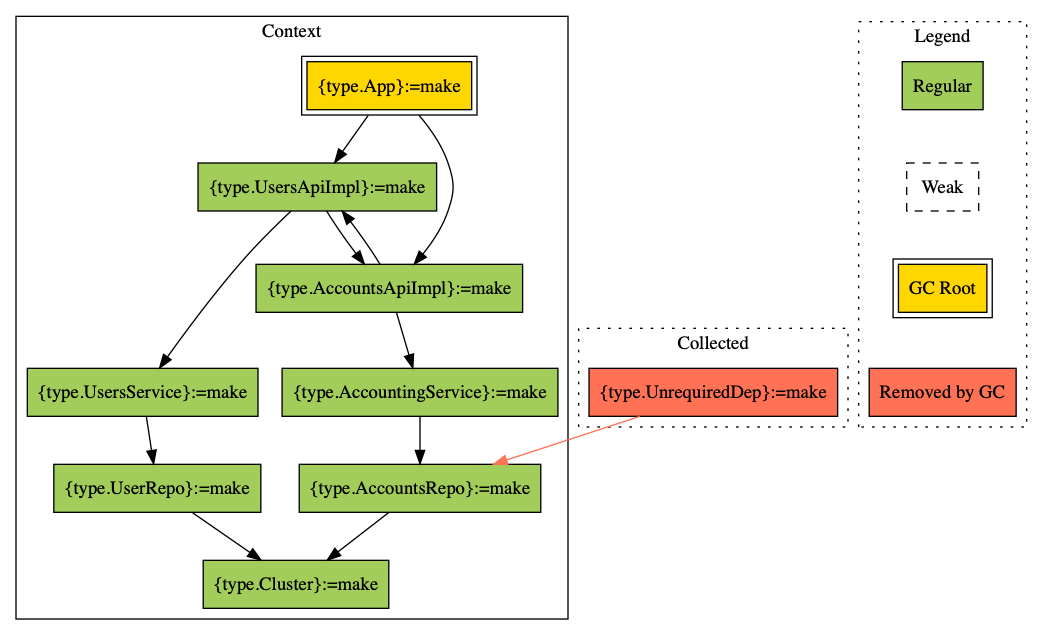
\includegraphics[width=\textwidth]{media/plan-example-dot}
  \end{figure}
  \footnotetext[1]{Generated automatically by \texttt{GraphDumpObserver} distage extension}
\end{frame}

\begin{frame}[fragile]
\frametitle{Plan Introspection: plan dumps}
\begin{scalacode}
println(plan.render) // look for the circular dependency!
\end{scalacode}

\begin{figure}
    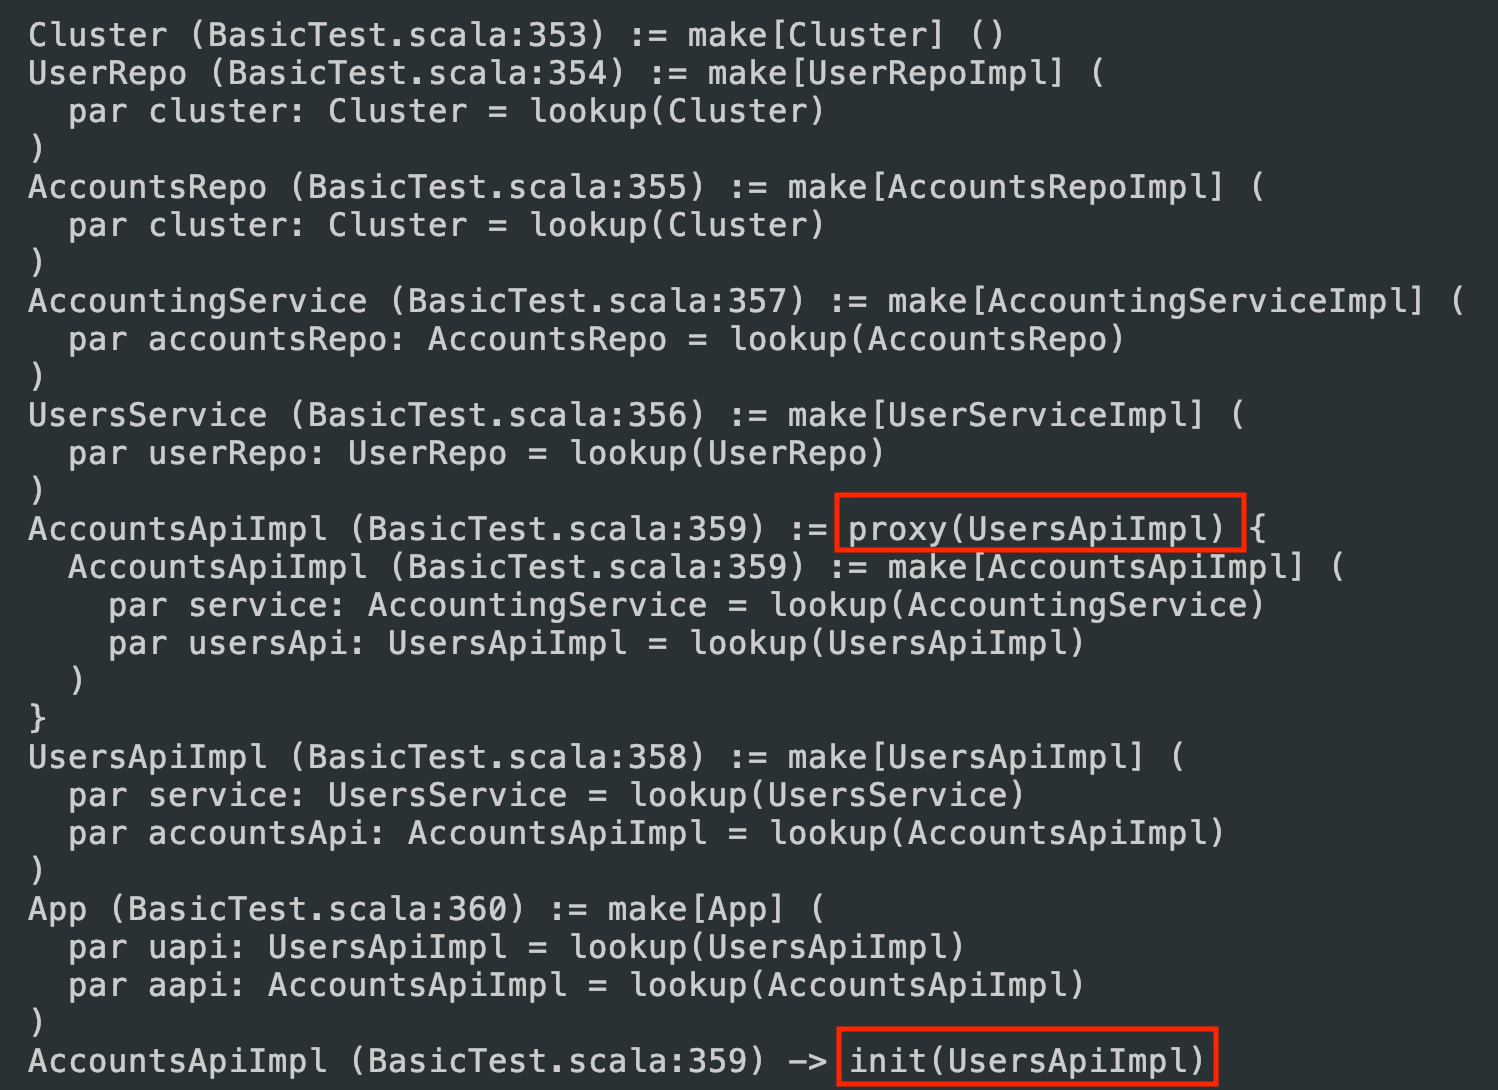
\includegraphics[width=0.75\textwidth]{media/plan-example.png}
\end{figure}
\end{frame}

\begin{frame}[fragile]
\frametitle{Plan Introspection: dependency trees}
You may explore dependencies of a component:

\begin{scalacode}
val dependencies = plan.topology.dependencies
println(dependencies.tree(DIKey.get[AccountsApiImpl]))
\end{scalacode}

\begin{figure}
    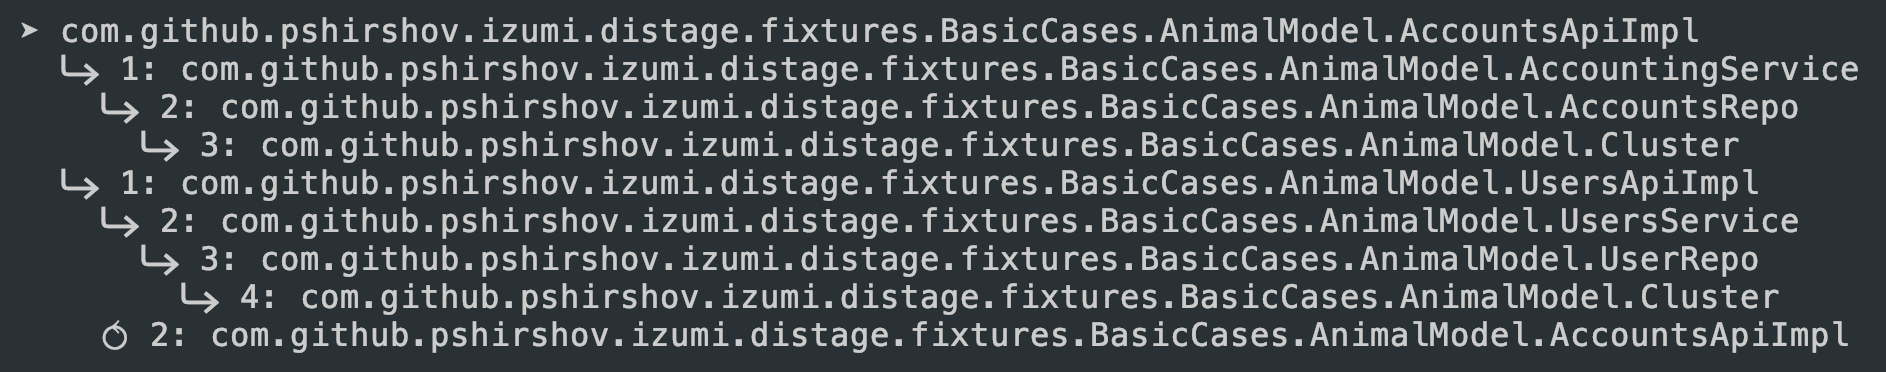
\includegraphics[width=\textwidth]{media/dependency-tree.png}
\end{figure}

Circular dependencies are marked with a circle symbol.
\end{frame}

\begin{frame}[fragile]
\begin{center}
\frametitle{Compile-Time and Runtime DI}
A Plan:
\begin{textcode}
myRepository := create[MyRepository]()
myservice    := create[MyService](myRepository)
\end{textcode}

May be interpreted as:

\begin{columns}

\begin{column}[T]{0.5\textwidth}
   \setlength{\topsep}{0pt}
   \setlength{\partopsep}{0pt}
Code tree (compile-time):
\begin{scalacode}
val myRepository =
    new MyRepository()
val myservice =
    new MyService(myRepository)
\end{scalacode}
\end{column}

\begin{column}[T]{0.5\textwidth}
Set of instances (runtime):
\begin{scalacode}
plan.foldLeft(Context.empty) {
case (ctx, op) =>
    ctx.withInstance(
        op.key
        , interpret(action)
    )
}
\end{scalacode}
\end{column}

\end{columns}
\end{center}
\end{frame}

%%%%%%%%%%%%%%%%%%%%%%%%%%%%%%%%%%%%%%%%%%%%%%%%%%%%%%%%%%%%%%%%%%%%%%%%%%%%%%%%%%%%%%%%%%%%%%%%%%%
\section{7mind stack}
\begin{frame}
  \begin{figure}
  \Huge
  \color{RubineRed} dist✪ge
  \noindent
  \rule{\linewidth}{1mm}
  \Large 7mind Stack
  \rule{\linewidth}{1mm}
  \end{figure}
\end{frame}

\begin{frame}[fragile]
  \frametitle{\distage: status and things to do}
  \distage{} 0.7:
  \begin{enumerate}
    \item is ready to use,
    \item is in production for over 1 year,
    \item has all runtime features available,
    \item has all compile-time features available except for full compile-time mode.
  \end{enumerate}
  \vspace{0.3cm}
  What's next:
  \begin{enumerate}
    \item New Resource-based Roles API,
    \item Scala.js support,
    \item Compile-time Producer,
    \item Isolated Classloaders for Roles (in future),
    \item Check our GitHub: https://github.com/pshirshov/izumi-r2.
  \end{enumerate}
\end{frame}

\begin{frame}
  \frametitle{\distage is just a part of our stack}
  We have a vision backed by our tools:
  \begin{enumerate}
    \item Idealingua: transport and codec agnostic gRPC alternative with rich modeling language,
    \item LogStage: zero-cost structured logging framework,
    \item \textit{Fusional Programming and Design} guidelines. We love both FP and OOP,
    \item \textit{Continous Delivery} guidelines for Role-based process,
    \item \textit{Percept-Plan-Execute} Generative Programming approach, abstract machine and computational model.
    Addresses Project Planning (see Operations Research). Examples: orchestration, build systems.
        %  Roles: distributed development without distributed computing
  \end{enumerate}

  Altogether these things already allowed us to significantly reduce development costs and
  delivery time for our client.\newline

  More slides to follow.
\end{frame}

\begin{frame}
  \begin{center}
  \Huge
  You use \texttt{Guice}?

  Switch to \distage!

  %\begin{figure}
  %    
\includegraphics[width=0.35\textwidth]{media/haruhi.jpg}
  %\end{figure}
  \end{center}

    \center{
  \textit{``Given its native support for type classes and higher-kinded types -- both features indispensable to functional programming -- DI Stage is one of the leading dependency injection libraries out there. Bonus points for being built by a wicked-smart team that contributes to ZIO!''}
  }
  \newline
  \leftline{\textit{ --– John A. De Goes}}
\end{frame}

\begin{frame}[fragile]
  \frametitle{Teaser: LogStage}
  A simple logging call \dots
  \begin{scalacode}
log.info(s"$user logged in with $sessionId!")
  \end{scalacode}

  May be rendered as text:
  \newline
  \texttt{
  17:05:18 UserService.login user=John Doe logged in with sessionId=DEADBEEF!
  }
  \newline

  Or as structured JSON:
  \begin{jsoncode}
{
  "user": "John Doe",
  "sessionId": "DEADBEEF",
  "_template": "$user logged in with $sessionId!",
  "_location": "UserService.scala:265",
  "_context": "UserService.login",
}
  \end{jsoncode}
\end{frame}

\begin{frame}
    \frametitle{Thank you for your attention}

    \begin{center}
      distage website: https://izumi.7mind.io/

      We're looking for clients, contributors, adopters and colleagues ;)
    \end{center}

    About the author:
    \begin{enumerate}
        \item coding for 19 years, 12 years of hands-on commercial engineering experience,
        \item has been leading a cluster orchestration team in Yandex, ``the Russian Google'',
        \item Created ``\textit{Yandex Interstellar Spaceship}'' -- an orchestration solution to manage 50K+ physical machines across 6 datacenters,
        \item Owns an Irish R\&D company, https://7mind.io,
        \item Contact: team@7mind.io,
        \item Github: https://github.com/pshirshov
        \item Slides: https://github.com/7mind/slides/
    \end{enumerate}
\end{frame}

\end{document}
